\documentclass[11pt, a4paper]{article}\usepackage[]{graphicx}\usepackage[]{color}
%% maxwidth is the original width if it is less than linewidth
%% otherwise use linewidth (to make sure the graphics do not exceed the margin)
\makeatletter
\def\maxwidth{ %
  \ifdim\Gin@nat@width>\linewidth
    \linewidth
  \else
    \Gin@nat@width
  \fi
}
\makeatother

\definecolor{fgcolor}{rgb}{0.251, 0.251, 0.251}
\newcommand{\hlnum}[1]{\textcolor[rgb]{0.502,0.086,1}{#1}}%
\newcommand{\hlstr}[1]{\textcolor[rgb]{1,0.4,0.2}{#1}}%
\newcommand{\hlcom}[1]{\textcolor[rgb]{1,0.251,0.502}{#1}}%
\newcommand{\hlopt}[1]{\textcolor[rgb]{0.251,0.251,0.251}{#1}}%
\newcommand{\hlstd}[1]{\textcolor[rgb]{0.251,0.251,0.251}{#1}}%
\newcommand{\hlkwa}[1]{\textcolor[rgb]{0.941,0.188,0.816}{#1}}%
\newcommand{\hlkwb}[1]{\textcolor[rgb]{0,0.439,0.902}{#1}}%
\newcommand{\hlkwc}[1]{\textcolor[rgb]{0.188,0.941,0.314}{#1}}%
\newcommand{\hlkwd}[1]{\textcolor[rgb]{0.69,0.188,0.941}{#1}}%

\usepackage{framed}
\makeatletter
\newenvironment{kframe}{%
 \def\at@end@of@kframe{}%
 \ifinner\ifhmode%
  \def\at@end@of@kframe{\end{minipage}}%
  \begin{minipage}{\columnwidth}%
 \fi\fi%
 \def\FrameCommand##1{\hskip\@totalleftmargin \hskip-\fboxsep
 \colorbox{shadecolor}{##1}\hskip-\fboxsep
     % There is no \\@totalrightmargin, so:
     \hskip-\linewidth \hskip-\@totalleftmargin \hskip\columnwidth}%
 \MakeFramed {\advance\hsize-\width
   \@totalleftmargin\z@ \linewidth\hsize
   \@setminipage}}%
 {\par\unskip\endMakeFramed%
 \at@end@of@kframe}
\makeatother

\definecolor{shadecolor}{rgb}{.97, .97, .97}
\definecolor{messagecolor}{rgb}{0, 0, 0}
\definecolor{warningcolor}{rgb}{1, 0, 1}
\definecolor{errorcolor}{rgb}{1, 0, 0}
\newenvironment{knitrout}{}{} % an empty environment to be redefined in TeX

\usepackage{alltt}
\usepackage{graphicx, color, fancyhdr, lastpage, bm, amsmath, multirow, colortbl, setspace, url, ulem, hyperref, rotating, subfigure, lineno, currfile,longtable,ctable,lscape,geometry}
\IfFileExists{upquote.sty}{\usepackage{upquote}}{}
\begin{document}


\title{A Minimal Demo of connect3}
\author{Chunqiao Luo}
\maketitle

\section{Introduction}
Package 'connect3' converts LaTeX files (with extension .tex) generated by R Sweave using package 'knitr' o Rich Text Format (RTF) files. Features include: 
\begin{itemize}
\item conversion of R syntax highlighting
\item conversion of tables generated by Hmisc::describe, Hmisc::summary, and Hmisc::latex
\item conversion of mathematical equations
\item conversion of graphics
\item conversion of itemize and enumerate
\item conversion of references
\end{itemize}

\section{Table}
\begin{knitrout}
\definecolor{shadecolor}{rgb}{0.973, 0.973, 0.973}\color{fgcolor}\begin{kframe}
\begin{alltt}
\hlcom{#Data Generation}
\hlkwd{set.seed}\hlstd{(}\hlnum{123}\hlstd{)}
\hlstd{StudyID}\hlkwb{<-}\hlkwd{seq}\hlstd{(}\hlnum{1}\hlopt{:}\hlnum{100}\hlstd{)}
\hlstd{gender}\hlkwb{<-}\hlkwd{rep}\hlstd{(}\hlkwd{c}\hlstd{(}\hlstr{"Male"}\hlstd{,}\hlstr{"Female"}\hlstd{),}\hlkwc{times}\hlstd{=}\hlnum{50}\hlstd{)}
\hlstd{age}\hlkwb{<-}\hlkwd{rnorm}\hlstd{(}\hlnum{100}\hlstd{,}\hlkwc{mean}\hlstd{=}\hlnum{10.00}\hlstd{,}\hlkwc{sd}\hlstd{=}\hlnum{1.50}\hlstd{)}
\hlstd{treatment}\hlkwb{<-}\hlkwd{rep}\hlstd{(}\hlkwd{c}\hlstd{(}\hlstr{'Yes'}\hlstd{,}\hlstr{'No'}\hlstd{),}\hlkwc{times}\hlstd{=}\hlnum{50}\hlstd{)}
\hlstd{race}\hlkwb{<-}\hlkwd{rep}\hlstd{(}\hlkwd{c}\hlstd{(}\hlstr{"Hispanic"}\hlstd{,}\hlstr{"White"}\hlstd{,}\hlstr{"Black"}\hlstd{,}\hlstr{"Other"}\hlstd{),}\hlkwc{times}\hlstd{=}\hlnum{25}\hlstd{)}
\hlstd{qolScore} \hlkwb{<-}\hlkwd{rnorm}\hlstd{(}\hlnum{100}\hlstd{,}\hlkwc{mean}\hlstd{=}\hlnum{70.0}\hlstd{,}\hlkwc{sd}\hlstd{=}\hlnum{10.0}\hlstd{)}
\hlstd{data}\hlkwb{<-}\hlkwd{data.frame}\hlstd{(}\hlkwc{StudyID}\hlstd{=StudyID,}
                 \hlkwc{gender}\hlstd{=gender,}
                 \hlkwc{age}\hlstd{=}\hlkwd{as.numeric}\hlstd{(age),}
                 \hlkwc{treatment}\hlstd{=}\hlkwd{factor}\hlstd{(treatment,} \hlkwd{c}\hlstd{(}\hlstr{'Yes'}\hlstd{,}\hlstr{'No'}\hlstd{)),}
                 \hlkwc{race}\hlstd{=}\hlkwd{factor}\hlstd{(race,} \hlkwd{c}\hlstd{(}\hlstr{"White"}\hlstd{,}\hlstr{"Black"}\hlstd{,} \hlstr{"Hispanic"}\hlstd{,}\hlstr{"Other"}\hlstd{)),}
                 \hlkwc{qolScore}\hlstd{=}\hlkwd{as.numeric}\hlstd{(qolScore))}
\hlkwd{str}\hlstd{(data)}
\end{alltt}
\begin{verbatim}
## 'data.frame':	100 obs. of  6 variables:
##  $ StudyID  : int  1 2 3 4 5 6 7 8 9 10 ...
##  $ gender   : Factor w/ 2 levels "Female","Male": 2 1 2 1 2 1 2 1 2 1 ...
##  $ age      : num  9.16 9.65 12.34 10.11 10.19 ...
##  $ treatment: Factor w/ 2 levels "Yes","No": 1 2 1 2 1 2 1 2 1 2 ...
##  $ race     : Factor w/ 4 levels "White","Black",..: 3 1 2 4 3 1 2 4 3 1 ...
##  $ qolScore : num  62.9 72.6 67.5 66.5 60.5 ...
\end{verbatim}
\begin{alltt}
\hlcom{#Summary Table}
\hlkwd{library}\hlstd{(Hmisc)}
\hlstd{Demo}\hlkwb{<-}\hlkwd{summary}\hlstd{(treatment}\hlopt{~}\hlstd{age}\hlopt{+}\hlstd{gender}\hlopt{+}\hlstd{race}\hlopt{+}\hlstd{qolScore,}\hlkwc{method}\hlstd{=}\hlstr{'reverse'}\hlstd{,} \hlkwc{test}\hlstd{=T)}
\hlstd{Demo}\hlkwb{<-}\hlkwd{latex}\hlstd{(Demo,} \hlkwc{size}\hlstd{=}\hlstr{'small'}\hlstd{,} \hlkwc{file}\hlstd{=}\hlstr{'Demo.tex'}\hlstd{,} \hlkwc{where}\hlstd{=}\hlstr{'!h'}\hlstd{)}
\end{alltt}
\end{kframe}
\end{knitrout}
%latex.default(cstats, title = title, caption = caption, rowlabel = rowlabel,     col.just = col.just, numeric.dollar = FALSE, insert.bottom = legend,     rowname = lab, dcolumn = dcolumn, extracolheads = extracolheads,     extracolsize = Nsize, ...)%
\begin{table}[!h]
{\small
\caption{Descriptive Statistics by treatment\label{Demo}} 
\begin{center}
\begin{tabular}{lccc}
\hline\hline
\multicolumn{1}{l}{}&\multicolumn{1}{c}{No}&\multicolumn{1}{c}{Yes}&\multicolumn{1}{c}{Test Statistic}\tabularnewline
&\multicolumn{1}{c}{{\scriptsize $N=50$}}&\multicolumn{1}{c}{{\scriptsize $N=50$}}&\tabularnewline
\hline
age&{\scriptsize  9.257589~}{10.018343 }{\scriptsize 10.944154} &{\scriptsize  9.296508~}{10.189856 }{\scriptsize 11.140469} &$ F_{1,98}=0.05 ,~ P=0.827 ^{1} $\tabularnewline
gender~:~Male&~~0\%~{\scriptsize~(~0)}&100\%~{\scriptsize~(50)}&$ \chi^{2}_{1}=100 ,~ P<0.001 ^{2} $\tabularnewline
race~:~Black&~0\%~{\scriptsize~(~0)}&50\%~{\scriptsize~(25)}&$ \chi^{2}_{3}=100 ,~ P<0.001 ^{2} $\tabularnewline
~~~~Hispanic&~0\%~{\scriptsize~(~0)}&50\%~{\scriptsize~(25)}&\tabularnewline
~~~~Other&50\%~{\scriptsize~(25)}&~0\%~{\scriptsize~(~0)}&\tabularnewline
~~~~White&50\%~{\scriptsize~(25)}&~0\%~{\scriptsize~(~0)}&\tabularnewline
qolScore&{\scriptsize 61.87878~}{67.28704 }{\scriptsize 73.08149} &{\scriptsize 62.25988~}{69.23240 }{\scriptsize 75.52094} &$ F_{1,98}=0.14 ,~ P=0.707 ^{1} $\tabularnewline
\hline
\end{tabular}\end{center}}

\noindent {\scriptsize $a$\ }{$b$\ }{\scriptsize $c$\ } represent the lower quartile $a$, the median $b$, and the upper quartile $c$\ for continuous variables.Numbers after percents are frequencies.\indent Tests used:\textsuperscript{\normalfont 1}Wilcoxon test; \textsuperscript{\normalfont 2}Pearson test\end{table}

\section{Figure}
\begin{knitrout}
\definecolor{shadecolor}{rgb}{0.973, 0.973, 0.973}\color{fgcolor}\begin{kframe}
\begin{alltt}
\hlkwd{hist}\hlstd{(data}\hlopt{$}\hlstd{qolScore,}\hlkwc{main}\hlstd{=}\hlstr{''}\hlstd{)}
\hlkwd{boxplot}\hlstd{(qolScore} \hlopt{~} \hlstd{treatment,} \hlkwc{data}\hlstd{=data)}
\end{alltt}
\end{kframe}

{\centering 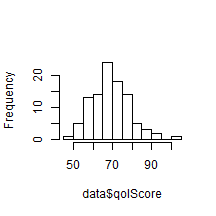
\includegraphics[width=.4\linewidth]{figure/minimal-plot-1} 
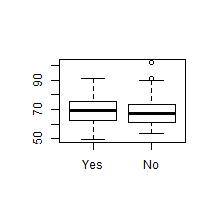
\includegraphics[width=.4\linewidth]{figure/minimal-plot-2} 

}



\end{knitrout}
\clearpage
\newpage

\begin{thebibliography}{2}

\bibitem{knitr 2015}
Yihui Xie (2015) knitr: A General-Purpose Package for Dynamic Report Generation in R. R package version 1.11.

\bibitem{Hmisc 2015}
Frank E Harrell Jr, with contributions from Charles Dupont and many others. (2015). Hmisc: Harrell Miscellaneous. R package version 3.16-0. http://CRAN.R-project.org/package=Hmisc
\end{thebibliography}
\end{document}
